\section{Performance Validation in Simulation - (Lead by Abhishek, Amelia, Lucian, Vlad)}\label{sec:mc}

To evaluate the performance of the MALTA2 quad-sensor module in the radiative
background expected near the beam-pipe at the Electron-Ion Collider (EIC), a
dedicated fast-simulation framework has been developed. The simulation is
based on a data-driven fast-simulation approach, in which the response
of the sensor is parameterized from MALTA2 sensor beam-test data rather than
from a detailed technology computer-aided design (TCAD) simulation. This parametric method reproduces the
charge-collection and timing behavior of the MALTA2 pixel with high accuracy, while remaining computationally efficient and therefore compatible to the simulation of high background environment and maybe used for multiple objective optimization in future studies i.e. detector placement, etc. The approach and its validation for MALTA2 sensors are
described in detailed Refs.~\cite{FastSim,MALTA2_CCParameterization}.

This section presents the simulation of the FMT telescope and the full analysis chain. The detector geometry, together with the generation of signal pions and the EIC beam-induced background, is described in Sec.~\ref{sec:geometry}. The digitization of the collected-charge, followed by tracking, clustering and the definition of the hit matching and efficiency criteria, is presented in Sec.~\ref{sec:reco}.
The timing performance of the module in the absence of background is discussed before the characterization of the EIC background rate and integrating in the simulation. Finally, the impact of the background rate on the hit efficiency of the MALTA2 sensors is quantified.

\subsection{Telescope geometry and setup in simulation}\label{sec:geometry}
The detector geometry, illustrated in Fig.~\ref{fig:geom}, consists of two quad-sensor modules placed parallel to each other along the beam direction ($z$). Each quad module comprises four MALTA2 sensors mounted side by side in the $xy$ plane, with a negligible gap of ${\approx}\,1\,\mu\mathrm{m}$ between adjacent sensors along $x$. The first module (Plane-0) is located at $z=0~mm$ and contains sensors S0--S3, while the second module (Plane~1), at $z=~100$~mm, contains sensors S100--S103. The sensor coordinates are listed in Table~\ref{tab:geom}. Each MALTA2 sensor is implemented in \textsc{Geant4} as a sensitive silicon volume of \SI{29.1}{\micro\meter} thickness. The sensor matrix comprises 512 columns along $x$ and 224 rows along $y$ with a pixel pitch of \SI{36.4}{\micro\meter}, corresponding to an active area of \SI{18.64}{\milli\meter} $\times$ \SI{8.15}{\milli\meter}. The readout timing propagates along the quad module from sensor S0 to S3 (and, analogously, from S100 to S103), corresponding to an \SI{8}{\nano\second} time offset between successive sensors. Both the electromagnetic and the hadronic physics lists are used in the simulation.

Signal particles are generated with a particle gun centered at $(18.64,\,0.0,\,-1000.0)$~mm, i.e. on the second sensor (S1/S101) of each plane, and are emitted in the longitudinal ($+z$) direction. The signal beam consists of mono-energetic \SI{1}{\giga\electronvolt/c} pions with zero transverse momentum.  
%\begin{equation}
%    D^{0} \rightarrow K^{-} \pi^{+}, \qquad \bar{D}^{0} \rightarrow K^{+} \pi^{-}.
%    \label{eq:d0decay}
%\end{equation}
%Positive charged Pions are used as signal particles since they are decay-products of $D^{0}$ as shown in Eq.~\ref{eq:d0decay} and that is one of benchmark for track reconstruction at EIC. (we need more rigrous justification)
The spatial distribution of the generated pion vertices follows a three-dimensional Gaussian distribution, with standard deviations of 0.5~mm in $x$ and $y$ and 100~mm in $z$ and it is shown in Fig.~\ref{fig:genXYZ}. The signal beam (charged particles) deposit energy in the Silicon sensor, and the two-dimensional distribution of raw hits is shown in Fig.~\ref{fig:rawhits2D}. The deposited energy is converted into charge using the data-driven fast-simulation method described in Ref.~\cite{FastSim}, whose charge-sharing model distributes the charge among the original pixel that got hit and its three nearest neighbours using an error-function width of \SI{4.3}{\micro\meter}~\cite{MALTA2_CCParameterization}. Along with charge collection, a parametric time-walk model is used to reproduce the realistic timing response of the MALTA2 sensor, as explained in Ref.~\cite{FastSim}. 


\subsection{Signal Reconstruction}\label{sec:reco}
The post-simulation analysis of \textsc{Geant4} simulated data proceeds in four following steps: digitization, tracking, clustering, and the final efficiency analysis. In the digitization step, the collected charge of each pixel is compared against a per-pixel threshold, and each hit passing the threshold is assigned a time given by the \textsc{Geant4} hit time plus a charge-dependent time-walk, a row-dependent propagation delay of \SI{12.5}{\pico\second} per row, the \SI{8}{\nano\second} per-sensor module delay described in Sec.~\ref{sec:geometry}, and a Gaussian jitter emulating the front-end and off-chip read-out noise. Each hit's spatial coordinate is encoded into a 40-bit word containing the pixel address, and any hits arriving within a \SI{1.6}{\nano\second} window are merged across the entire sensor matrix to replicate the asynchronous readout. These encoded words are then decoded back into spatial coordinates, defining the digitized (or reconstructed) hits (X,Y). Both the raw and the digitized hits are stored in separate ROOT files for further analysis. 

The particle gun generate signals in the interval of \SI{2}{\micro\second}~ ; although the EIC bunch-crossing interval is \SI{10.2}{\nano\second}, signal events are only produced every \SI{2}{\micro\second}~\cite{beamveto}. In the tracking step, signal particles are reconstructed across both sensor planes (Plane 0 \& Plane 1) and matched to the generated truth tracks in space and time window; a reconstructed hit( X,Y) is considered matched if it falls within a \SI{100}{\micro\meter} radius and a \SI{500}{\nano\second} time window relative to the generated truth track\footnote{As the beam is strictly normal to the sensor, truth tracks are obtained by directly extrapolating the generated vertices onto the sensor plane, allowing for a direct comparison with the reconstructed hits.}. During clustering, edge-connected pixels (excluding diagonals) that share charge and belong to the same truth track are grouped together to form a cluster, the cluster time is defined by the earliest hit in the cluster, and a row-corrected timing is obtained by subtracting the row-dependent propagation delay. Finally, the hit efficiency is defined as the number of reconstructed signal particles satisfying these matching criteria divided by the total number of generated signal particles. In the absence of background particles, the hit efficiency for \SI{1}{\giga\electronvolt/c} pions is ${\approx}~\SI{96.8}{\percent}$. This efficiency loss arises from multiple factors: first, a \SI{1}{\giga\electronvolt/c} pion has an ${\approx}\SI{1.6}{\percent}$ probability of decaying over the ${\approx}\SI{1000}{\milli\meter}$ distance between the particle gun and the sensor; second, charge shared across a 4-pixel cluster can drop individual pixel signals below the $200\,\text{e}^-$ threshold. Third, because the fully asynchronous readout organizes pixels into 
2×8 groups, hits arriving at the periphery within the same \SI{1.6}{\nano\second} window are merged to reduce data volume. However, when coincident hits originate from different pixel groups, this merging leads to hit displacement or loss, shifting the reconstructed hit outside the defined spatial matching window.



\begin{figure}[H]
    \centering
    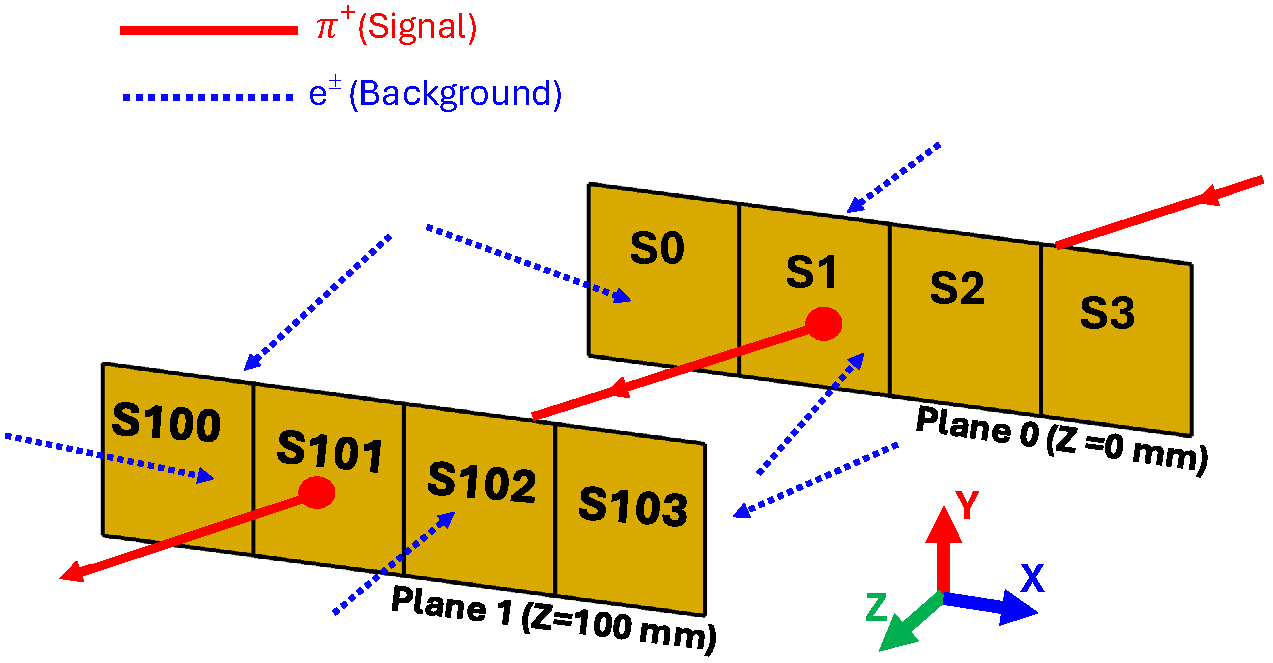
\includegraphics[width=0.5\textwidth]{Figures/geom.pdf}
    \caption{%
        MALTA2 QUAD Module geometry: eight $18.6 \times 8.15$~mm$^{2}$ silicon sensors in two planes separated by 100~mm.
        Red: \SI{1}{\giga\electronvolt/c} $\pi^{+}$ signal beam generated at $z = -1000$~mm and focused on the second sensor (S1 \& S101) of each plane.
        Blue dashed: randomly generated background $e^{\pm}$.
    }
    \label{fig:geom}
\end{figure}

\begin{table}[H]
    \centering
    \caption{%
        Positions of the eight MALTA2 sensors in the quad-module geometry.
        All sensors lie in the $y = 0$ plane and are placed side by side along $x$
         for Plane~0 (S0--S3) and Plane~1 (S100--S103).
    }
    \label{tab:geom}
    \begin{tabular}{c c c c c c}
        \hline
        Plane & $z$ [mm] & \multicolumn{4}{c}{Sensor $x$-centre [mm]} \\
        & & S0 / S100 & S1 / S101 & S2 / S102 & S3 / S103 \\
        \hline
        0 & 0   & 0.00 & 18.64 & 37.27 & 55.91 \\
        1 & 100 & 0.00 & 18.64 & 37.27 & 55.91 \\
        \hline
    \end{tabular}
\end{table}

\begin{figure}[H]
    \centering
    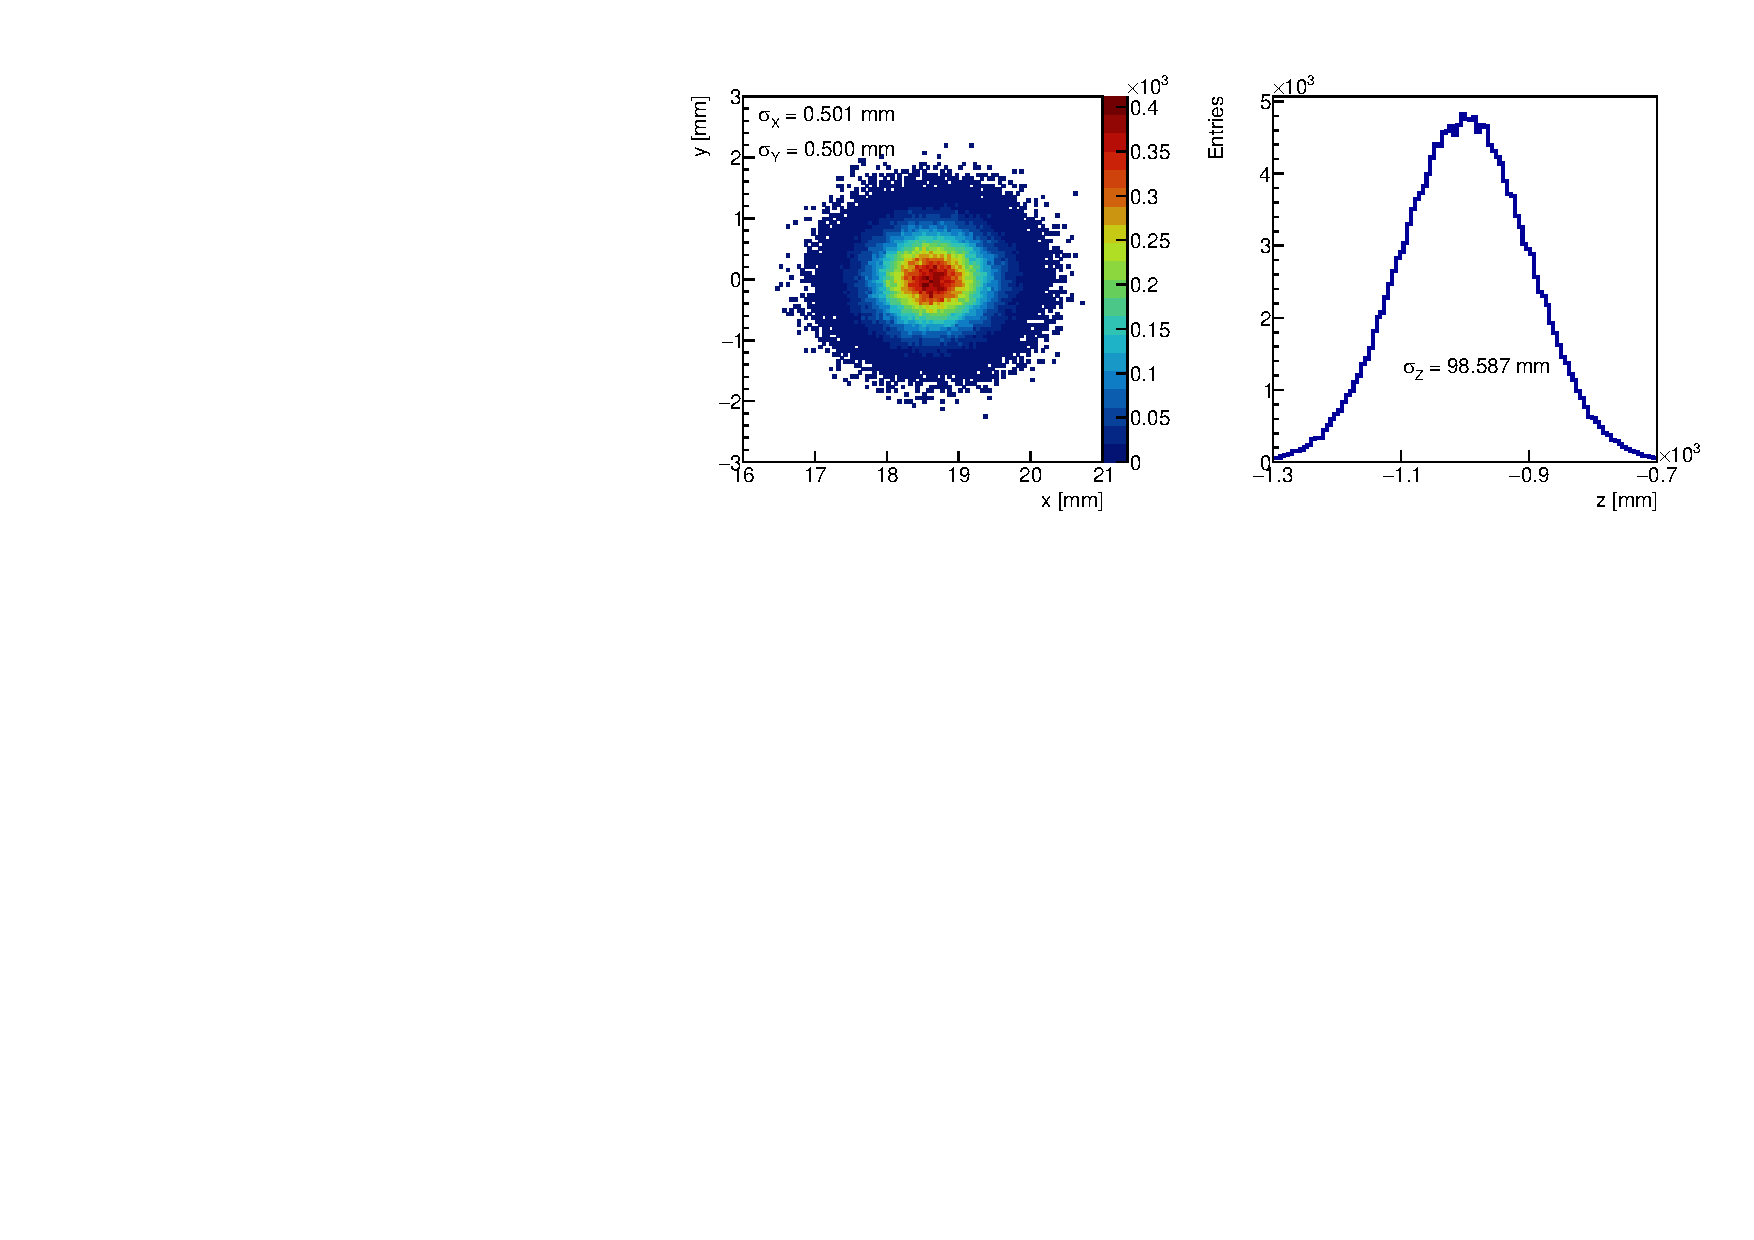
\includegraphics[width=\linewidth]{Figures/verify_gen_vertex.pdf}
    \caption{%
        Generated signal-beam vertex positions: (left) transverse $(x, y)$ distribution and (right) longitudinal $z$ distribution.
    }
    \label{fig:genXYZ}
\end{figure}


\begin{figure*}[t]
    \centering
    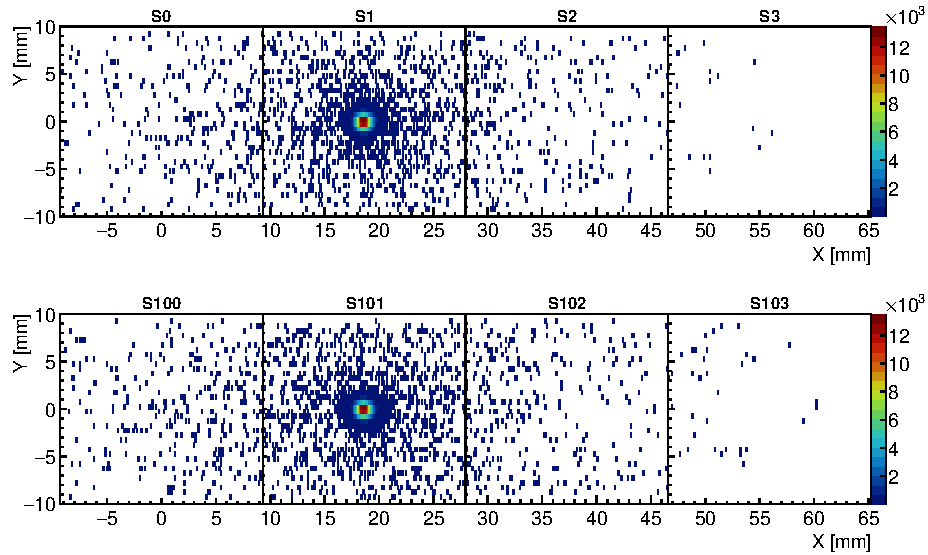
\includegraphics[width=\textwidth]{Figures/verify_2D_XY_both_planes.pdf}
    \caption{%
        Two-dimensional distribution of raw hits in the eight MALTA2 sensors.
        The top row shows sensors S0--S3 of the plane-0 and the bottom row sensors S100--S103 of the plane-1.
    }
    \label{fig:rawhits2D}
\end{figure*}

\subsection{Time Resolution (no background)}
The time resolution of the MALTA2 sensor is determined by storing the earliest hit time ($t_{0}$) of each cluster, which corresponds to the signal arrival and the sensor's response time (explained in Section \ref{sec:reco}). To compute the detector intrinsic time resolution, the core of the $t_{0}$ distribution is fitted with a Gaussian distribution, and the standard deviation of this fit defines the resolution for each sensor. The tails of the distribution are excluded from the fit because they exhibit non-Gaussian behavior primarily caused by \textcolor{red}{front-end electronics effects included in simulation}. The resulting time resolutions for the Plane 0 sensors (S0--S3) are illustrated in Fig.~\ref{fig:moduletime}.
The time resolution of each MALTA2 sensor is approximately 1.5 ns and peak of each sensor is separated by $\approx 8$~ns. Hence, simulated quad module reproduces the real quad-module MALTA2 sensor behavior. 
\begin{figure}
    \centering
    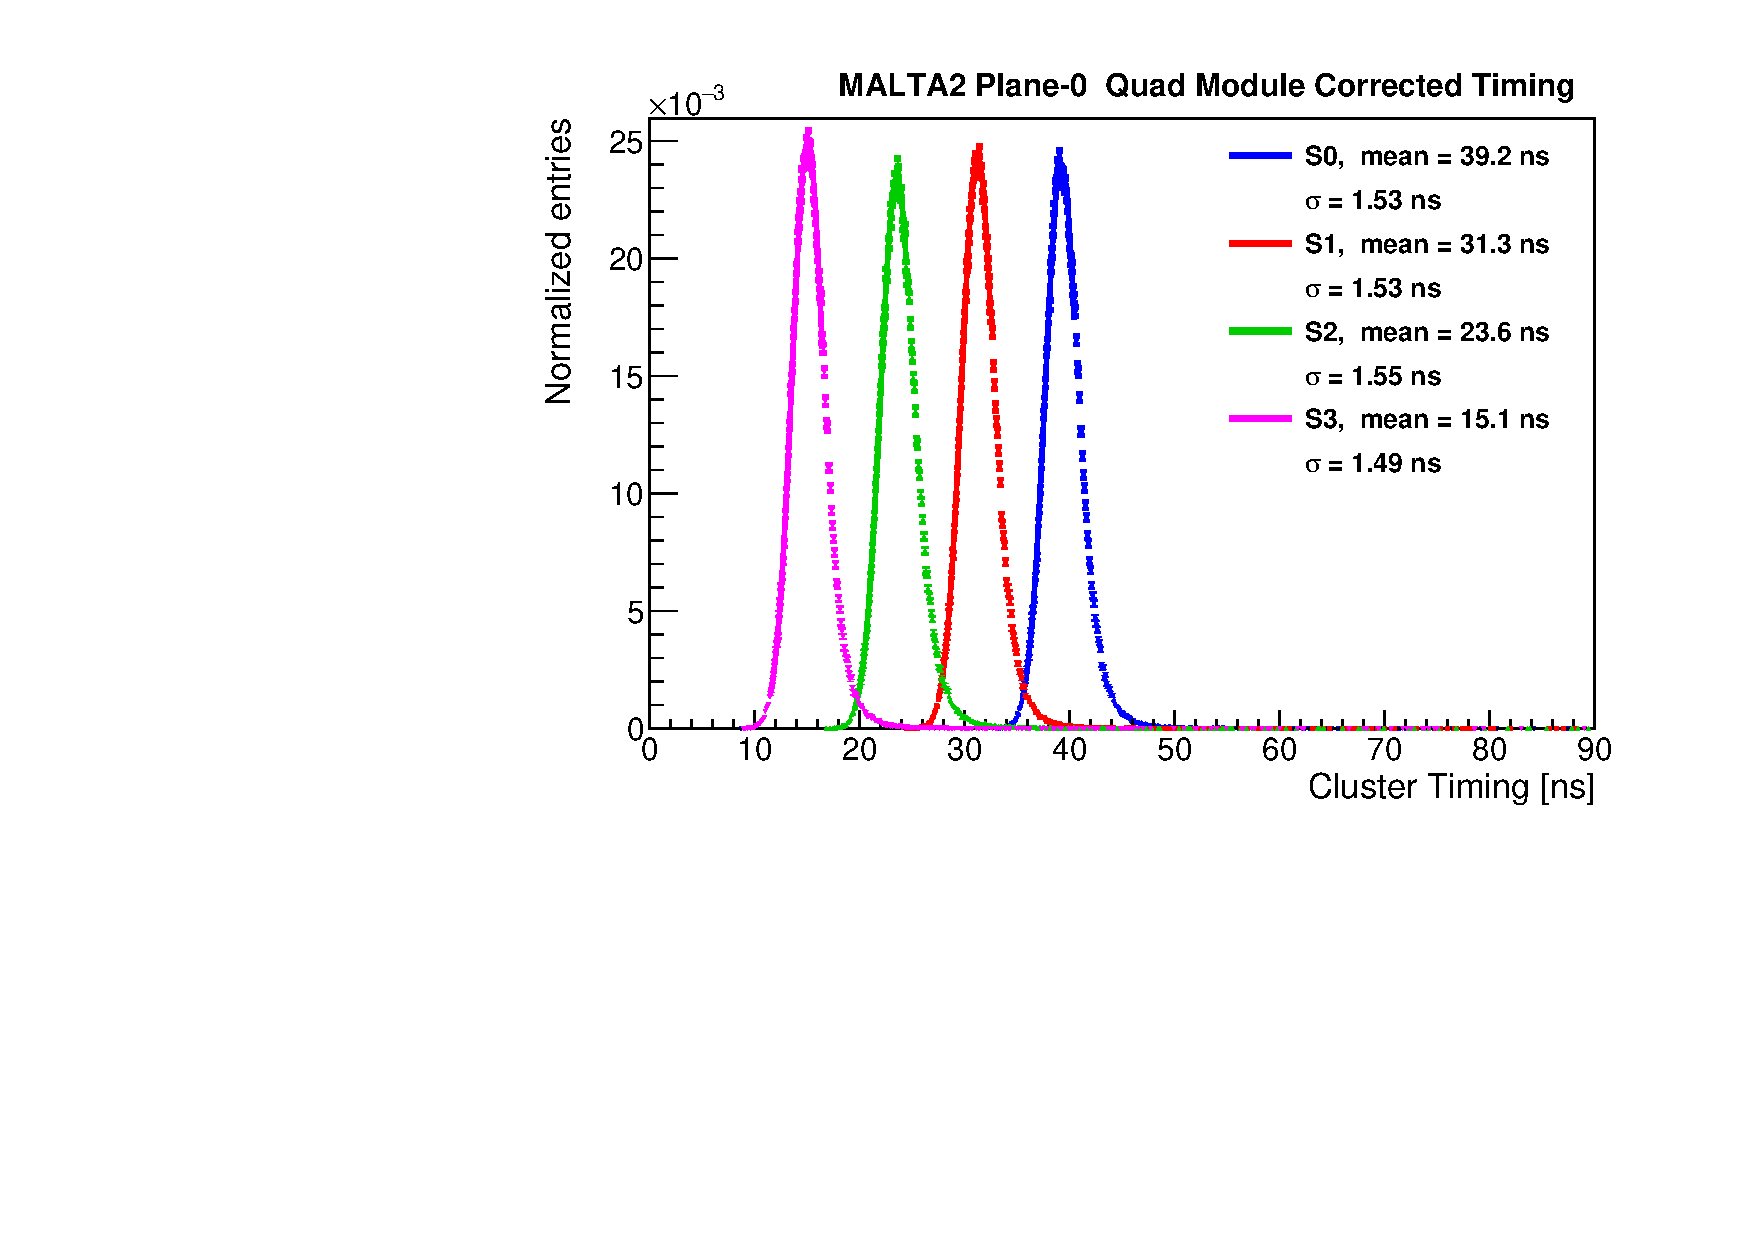
\includegraphics[width=\linewidth]{Figures/CorrectedTiming_all4.pdf}
    \caption{Cluster timing distribution of each sensor. Timing distribution is fit with Gaussian distribution. }
    \label{fig:moduletime}
\end{figure}
% \textcolor{red}{Plot: Time resolution (compare: without background, with 1,2,3 particles per event)}
% Validated with data.

\subsection{Background rate}\label{sec:BKGRATE}
% Explain the expected background at the location of the FMT (from Amelia's plots?):
% \begin{itemize}
%     \item Select region of $1\times\SI{2}{\square\centi\meter}$ with highest hit rate.
%     \item Show distribution of hits per $\SI{2}{\micro\second}$ event
%     \item Show PDG code of background particles. Is it primarily photons and electrons/ positrons?
% \end{itemize}

% Explain the simplifications/ assumptions that go into the MALTA2 simulation.
% \begin{itemize}
%     \item Identify maximum expected background hit rate per sampled event.
%     \item Spatial distribution is approximately flat within individual MALTA2 sensor.
% \end{itemize}

To determine the expected background rate, projected plots were made using the EIC simulation files alongside PyROOT analysis. The EIC GEANT4 simulation files used were the April 2026 FULL deep inelastic scattering neutral current background files. Since these were FULL files, each contained the Geant4 simulation ROOT files as well as truth level information. The reference location of 1415 mm from the point of collision was chosen to represent the environment near the proposed FMT location. By masking to the chosen z-location, it was possible to extract various background distributions at the disk location. In addition to the z-location “disk” mask, a “sensor” mask was applied to the disk as a way to isolate the footprint of one MALTA2 sensor within the disk. This “sensor” mask limited the x- and y- dimensions to that of one MALTA2 sensor with a final footprint of 1 by 2 $cm^{2}$.

To determine the peak background rate, the highest hit sensor was chosen out of several sensors near the beampipe. Because the hit and momentum distributions were of interest, the highest hit background sensor plots can be found in Fig. \ref{fig:expected_sensor_background} . The top left 2D histogram was used to determine the expected rate per event in the default 2 \(\mu s\) window by taking the integral of the plot. This resulted in an expected rate per event of 0.198. Additionally, this plot shows that the spatial distribution in this plot is relatively flat within an individual MALTA2 sensor.

An analysis of the background particle populations was also deemed important. By using the Monte Carlo particle information (PDG's), it was determined that the background near the proposed FMT location primarily consists of approximately 1\% positrons (PDG = -11), 37\% electrons (PDG = 11), and 48\% photons (PDG = 22).

\begin{figure*}[t]
    \centering
    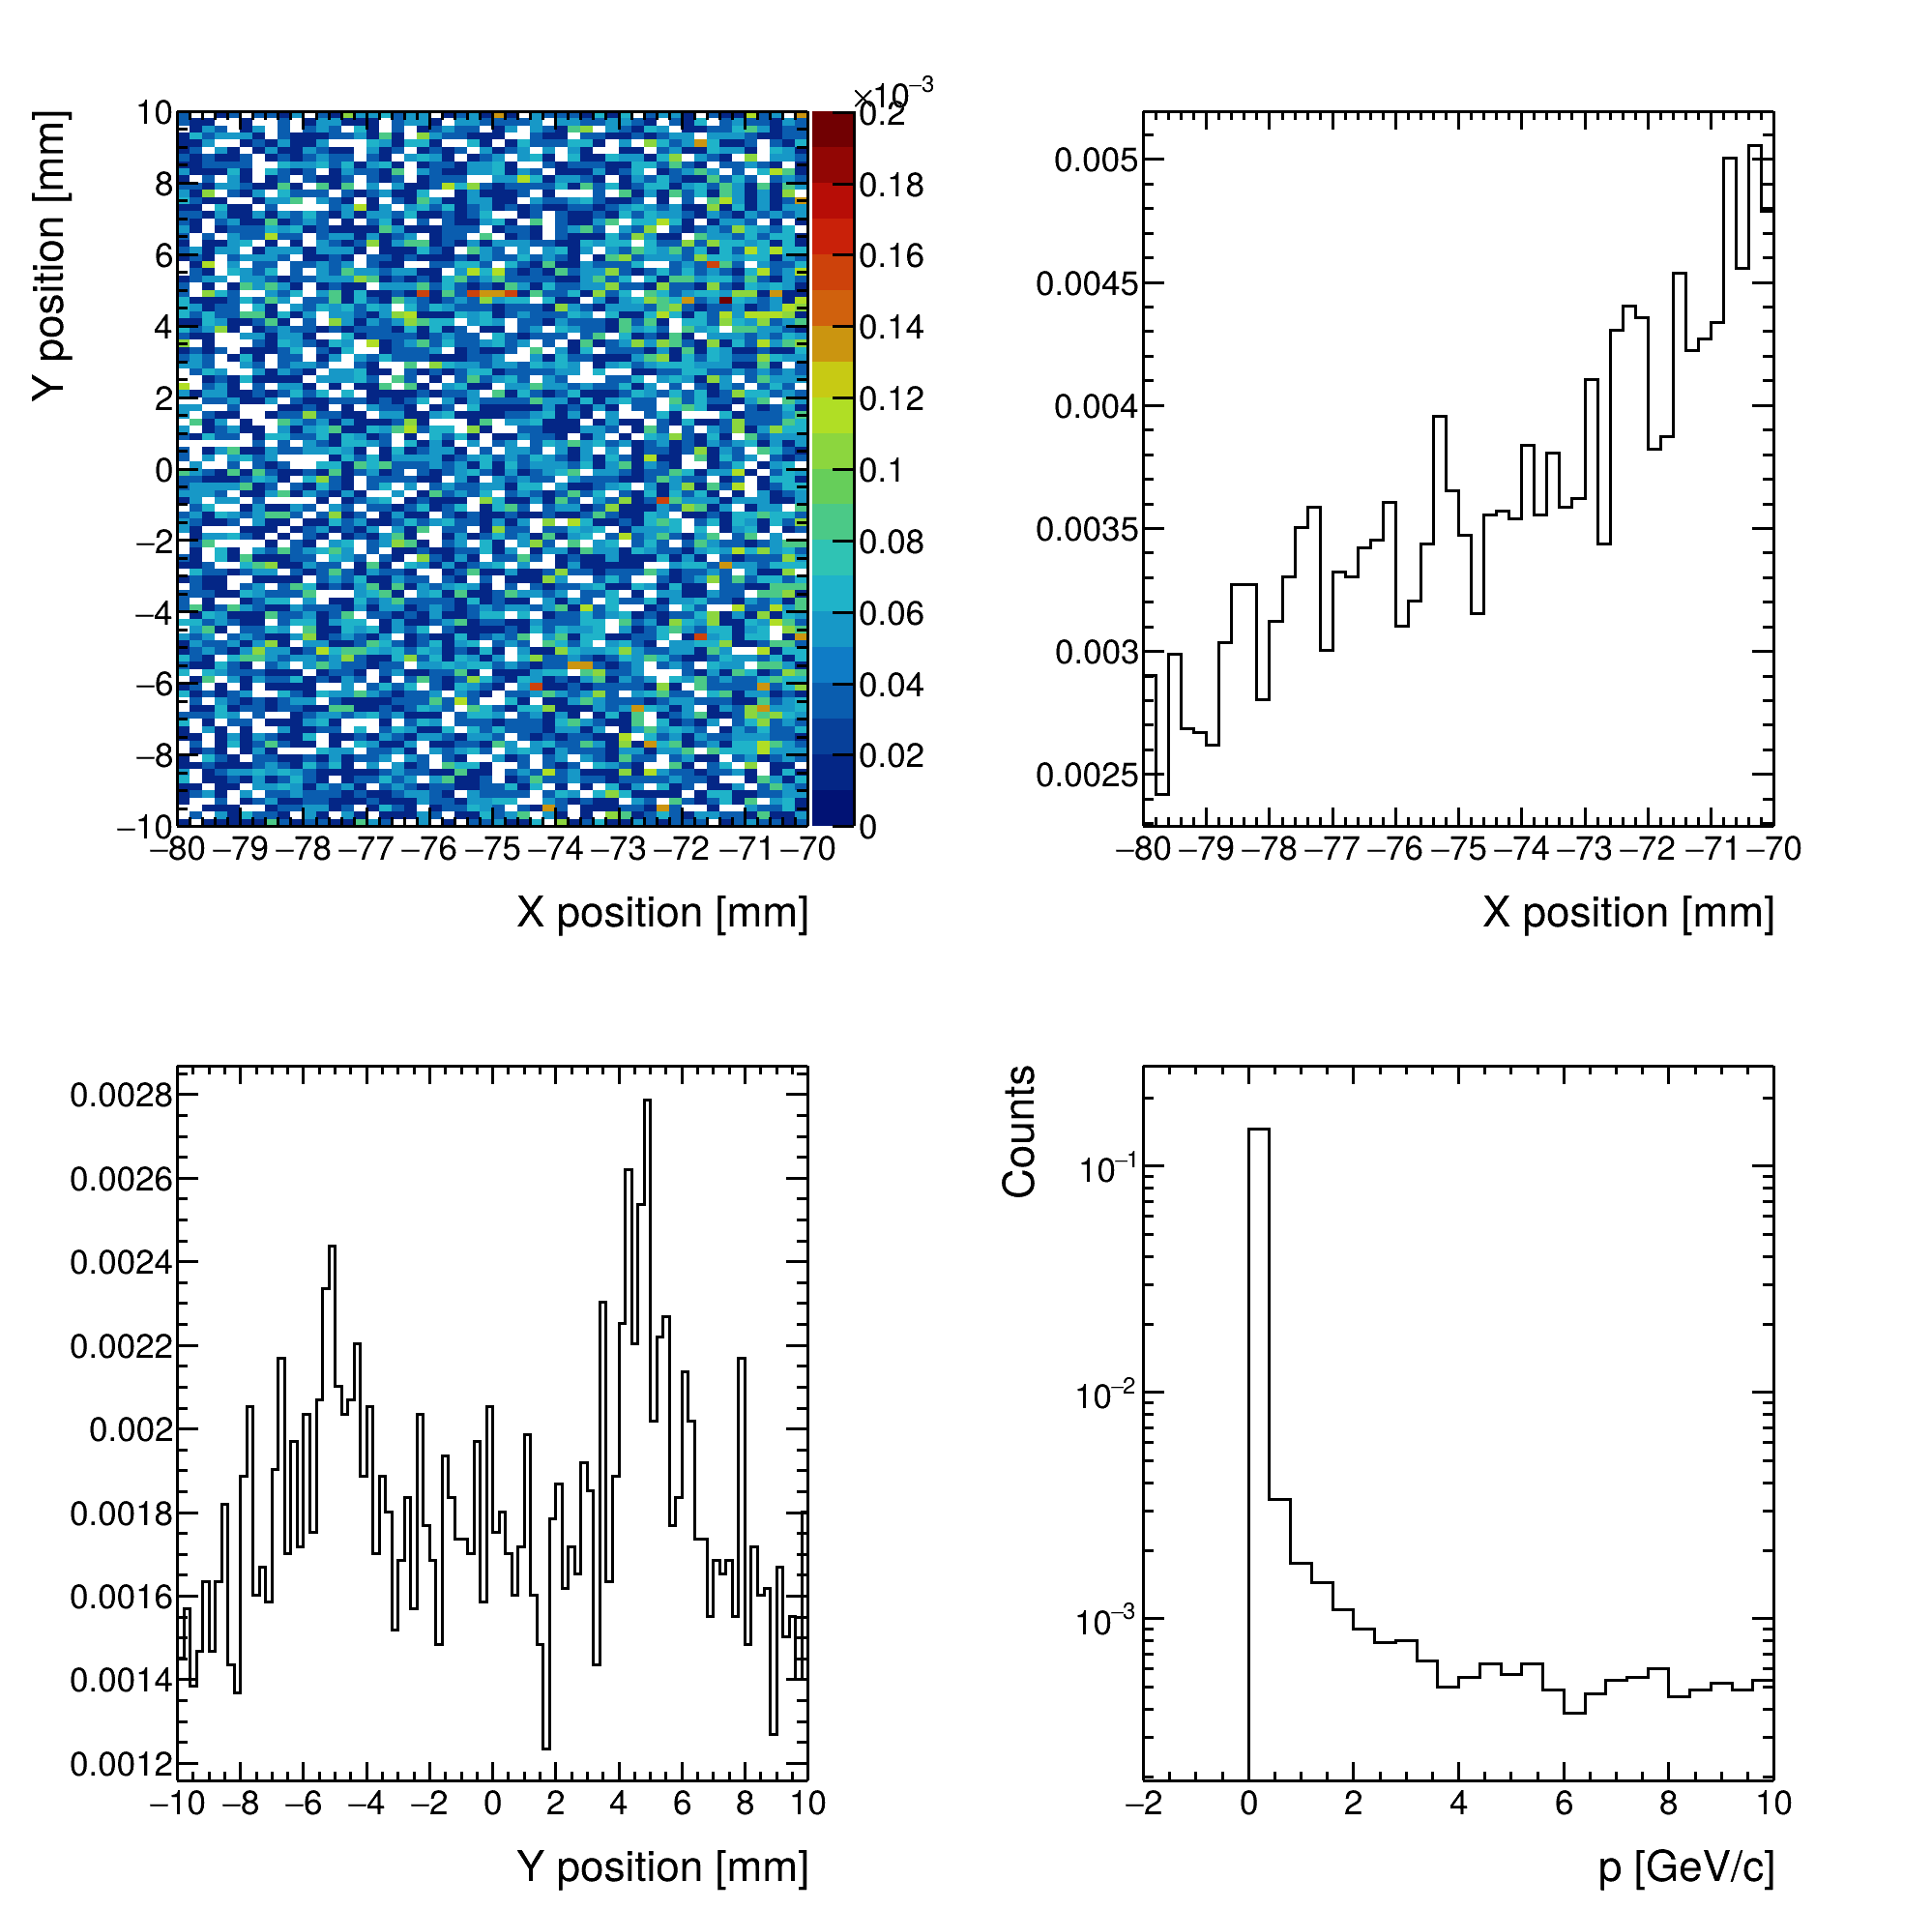
\includegraphics[width=\textwidth]{Figures/EIC_current_background_AprilFULL.png}
    \caption{Expected background distributions for a MALTA2 sensor at z = 1415 mm from the collision point. Far left: 2D histogram of hits in the x- and y- dimensions; Middle left: x-projection of hits; Middle Right: y-projection of hits; Far right: momentum magnitude distribution.}
    \label{fig:expected_sensor_background}
\end{figure*}

\subsection{Sampling of EIC Background}
For simulating the Electron-Ion Collider (EIC) background within each \SI{2}{\micro\second} time window, background electrons and positrons are generated by defining their momentum, spatial trajectory, and arrival rate. First, to reproduce the momentum distributions shown in Fig.~\ref{fig:expected_sensor_background}, the particle momentum magnitudes are parameterized using a Crystal Ball function. The resulting fit parameters are then used to randomly draw particle momenta via inverse-transform sampling; the corresponding fit for electrons is shown in Fig.~\ref{fig:bkgCB}. Second, the starting positions (vertices) of the particles are distributed uniformly at random within a three-dimensional box spanning the simulation world volume ($\SI{2}{\meter} \times \SI{2}{\meter} \times \SI{6}{\meter}$). Their trajectories are constrained to intersect at least one of the two quad-modules (Plane-0 or Plane-1) at a random sensor (Fig.~\ref{fig:geom}). Finally, the number of background particles generated per \SI{2}{\micro\second} window is sampled from a Poisson distribution across varying mean rates ($\lambda$). For reference, the nominal EIC background rate is ${\approx}\,1.5$ particles per \SI{2}{\micro\second} per MALTA2 sensor. Because the detector geometry comprises eight sensors in total, the single-sensor rate is scaled by a factor of eight to represent the full telescope coverage.


\begin{figure}[H]
    \centering
    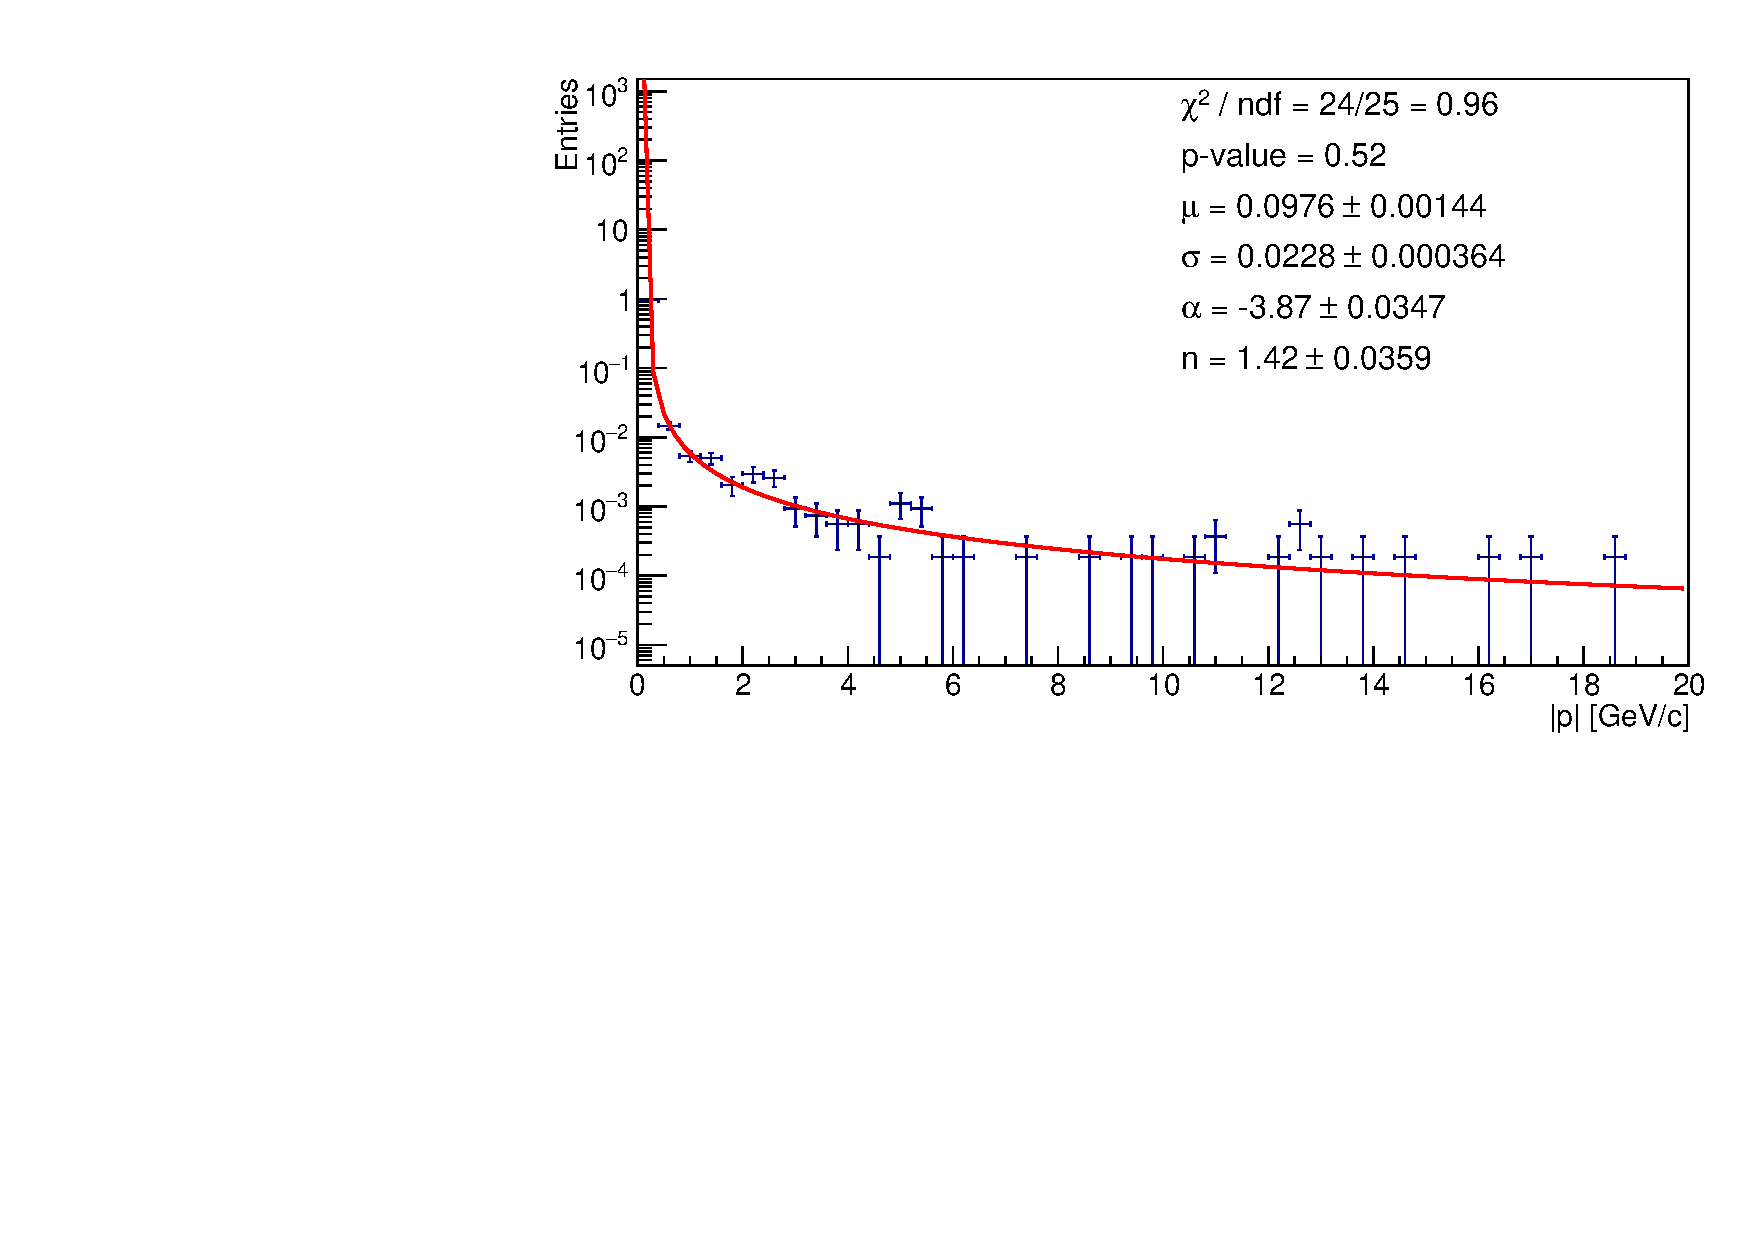
\includegraphics[width=\linewidth]{Figures/electron_cb_par_pmag.pdf}
    \caption{%
        Crystal Ball fit to the momentum magnitude distribution of background electrons.
    }
    \label{fig:bkgCB}
\end{figure}

\subsection{Hit efficiency with background}
To quantify the ability of the FMT to reconstruct signal tracks in the presence of beam induced background, the background rate $\lambda$ is varied from 0 to 15.84 particles per \SI{2}{\micro\second} window, i.e. up to ten times the nominal EIC background rate of $\lambda_{\mathrm{EIC}} \approx 1.584$ particles
per window summed over the eight sensors. At each rate the signal beam,
consisting of \SI{1}{\giga\electronvolt/c} pions at normal incidence,
is directed onto sensors S1 and S101, and the hit efficiency is
measured, as shown in Fig.~\ref{fig:bkgEff}.

The per-plane hit efficiency is defined as the fraction of signal pions
that satisfy the hit-matching criteria described in Sec.~\ref{sec:reco}
within a given plane. Both planes shows a slow, nearly linear decrease
of the hit efficiency with increasing background rate, with plane 1 lower by approximately \SI{1}{\percent} because a small
fraction of pions scatter in the first sensor layer. The coincidence
efficiency, which requires a reconstructed hit in both planes within an
\SI{36}{\nano\second} coincidence window, is lower than either per-plane
efficiency, and decreases faster with background rate. Two mechanisms
contribute to this: first, pions scattered in the first sensor layer are
displaced in the second plane, so a small fraction of events fail the
coincidence requirement as the occupancy increases; second, background
hits arriving within the \SI{1.6}{\nano\second} word-encoding window can
corrupt or displace the signal hit, further reducing the efficiency. The
measured efficiencies confirm that the MALTA2 sensors retain high
reconstruction efficiency up to several times the nominal EIC background
rate, demonstrating the feasibility of the FMT in the presence of background.

\begin{figure}[H]
    \centering
    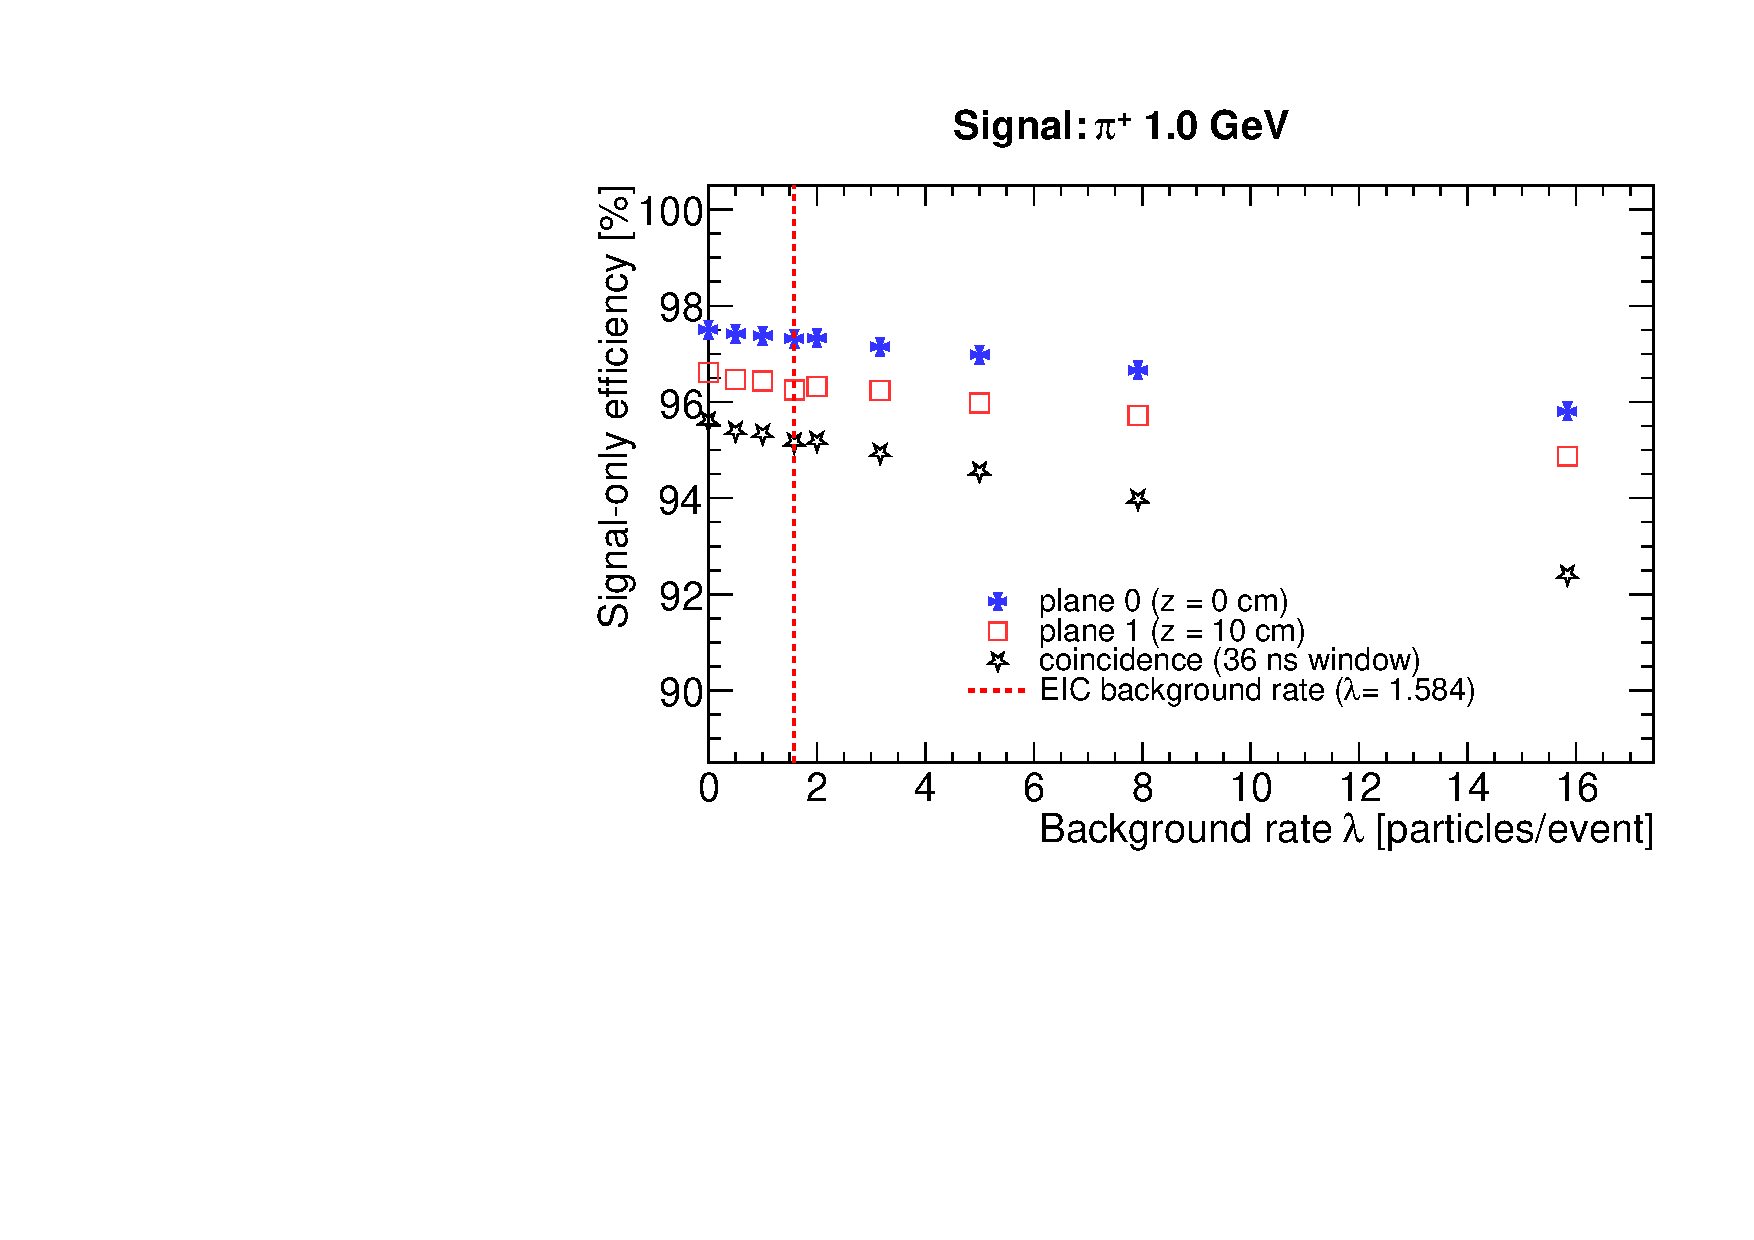
\includegraphics[width=\linewidth]{Figures/bkg_eff.pdf}
    \caption{%
        Hit efficiency as a function of the background rate for 1~GeV pions.
        Per-plane efficiencies are shown for plane 0 and plane 1, together with the coincidence efficiency.
    }
    \label{fig:bkgEff}
\end{figure}

\begin{figure}[H]
    \centering
    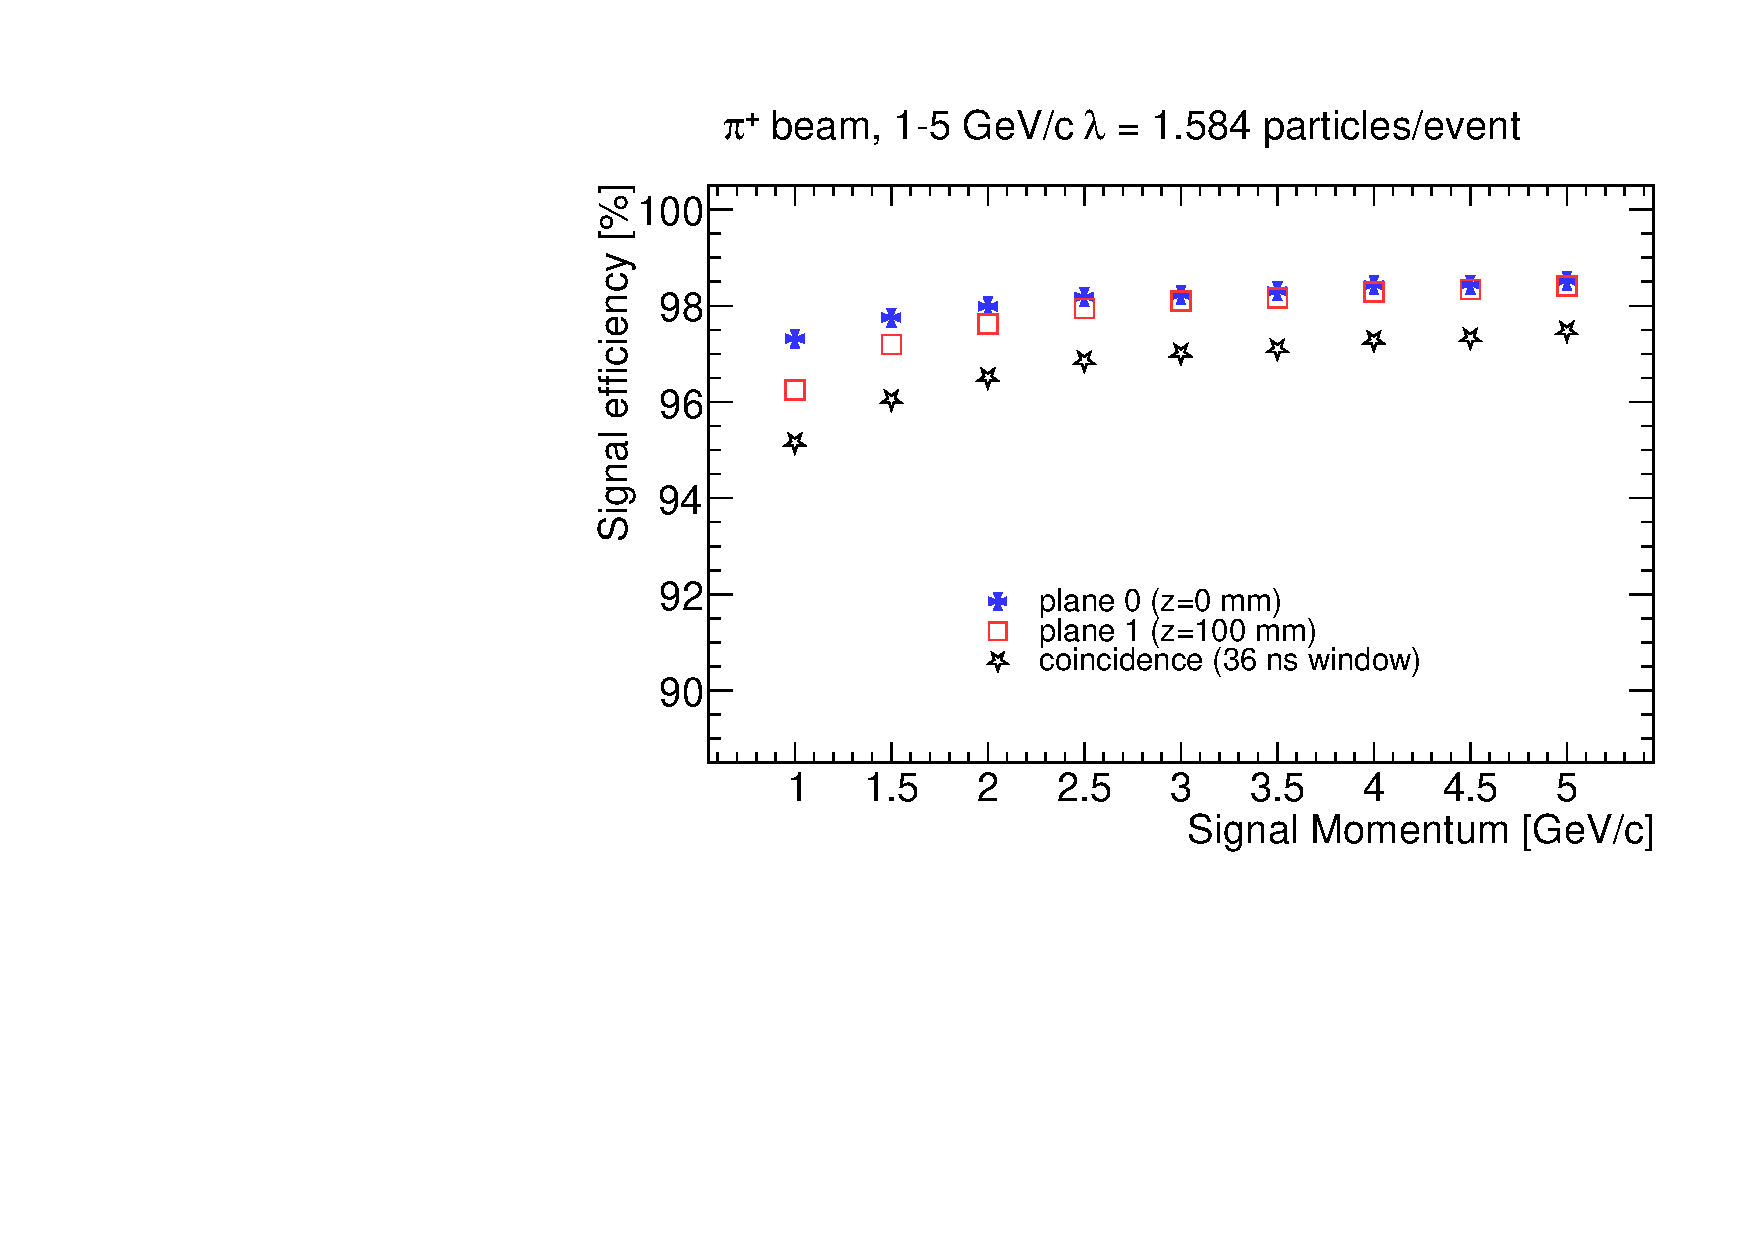
\includegraphics[width=\linewidth]{Figures/eff_vs_energy.pdf}
    \caption{%
        Hit efficiency as a function of the signal momentum.
        Background rate is fixed at EIC background rate $\lambda = 1.584~\mathrm{particles/event}$. 
    }
    \label{fig:effvsenergy}
\end{figure}


% \subsection{Tracking efficiency, potential spatial/temporal resolution with background}
% This subsection can target the proper tracking efficiency using 2 FMT planes.
% \begin{itemize}
%     \item Obtain hits per plane.
%     \item Reconstruct a track from the two planes.
%     \item Calculate pointing resolution of the track. In the simulation, signal is incident perpendicular onto the sensor. How is the direction reconstructed from the track?
% \end{itemize}

% \subsection{Matching capability with background}
